\documentclass[]{article}
\usepackage{graphicx}
\usepackage{grffile}
\usepackage{float}
\usepackage[language= italian, backend= biber, style=numeric]{biblatex}
\usepackage[italian]{babel}
\usepackage{guit}
\usepackage[utf8]{inputenc}
\usepackage{amsmath}
\usepackage{csquotes}
\usepackage{tikz}
\usepackage[italian]{hyperref}
\usetikzlibrary{shapes.geometric, arrows}
\tikzstyle{startstop} = [rectangle, rounded corners, minimum width=3cm, minimum height=1cm,text centered, draw=black, fill=red!30]
\tikzstyle{io} = [trapezium, trapezium left angle=70, trapezium right angle=110, minimum width=3cm, minimum height=1cm, text centered, draw=black, fill=blue!30]
\tikzstyle{process} = [rectangle, minimum width=3cm, minimum height=1cm, text centered, draw=black, fill=orange!30]
\tikzstyle{decision} = [diamond, minimum width=3cm, minimum height=1cm, text centered, draw=black, fill=green!30]
\tikzstyle{arrow} = [thick,->,>=stealth]

\hypersetup{%
	pdfpagemode={UseOutlines},
	bookmarksopen,
	pdfstartview={FitH},
	colorlinks,
	linkcolor={black}, %COLORE DEI RIFERIMENTI AL TESTO
	citecolor={blue}, %COLORE DEI RIFERIMENTI ALLE CITAZIONI
	urlcolor={blue} %COLORI DEGLI URL
}

\addbibresource{bibesame.bib}
\DeclareNameAlias{default}{last-first}

%opening
\title{BBC Buiness Articles text exploration and benchmark bulding for Automatic Topic Modeling evaluation}
\author{Tommaso Di Vincenzo, 801487\footnote{t.divincenzo@campus.unimib.it} \and Riccardo Maganza, 808053\footnote{r.maganza@campus.unimib.it}}


\begin{document}
\renewcommand{\abstractname}{Abstract}

\maketitle

\begin{abstract}
Nel paper viene condotta un'analisi su un corpus di 510 articoli di business in lingua inglese. Il fine è quello di confrontare le performance di riconoscimento dei topics individuati dal modello \textit{Latent Dirichlet Allocation} (LDA) con quelle derivanti da una suddivisione per argomenti creata manualmente a partire da un clustering ottenuto con l'algoritmo dei k-medoidi. Viene successivamente analizzata la coerenza semantica dei topics individuati attraverso la Normalized Google Distance (NGD). I risultati sono incoraggianti: le performance dell'algoritmo automatico sono molto vicine al benchmark ed in alcuni casi lo superano. Si discutono inoltre le applicazioni metodologiche di questi risultati. \footnote{Tutto il codice è disponibile su \url{https://gitlab.com/xelmagax/TextMiningBBCBusiness}}
\end{abstract}

\section{Introduzione}
L'estrazione di parole chiave da un testo è un'abilit\`a innata per gli umani, che sono in grado di distinguere con molta chiarezza ciò che è importante da ciò che può passare in secondo piano. \newline
In tempi moderni la quantità di dati disponibili sotto forma di documenti non strutturati è aumentata esponenzialmente, e con essa la difficoltà nel conservare questi testi ed indicizzarli. Se precedentemente categorizzare ogni documento manualmente in fase di caricamento, in un qualche tipo di database, poteva essere una possibilità, oggigiorno ciò sembra alquanto proibitivo. \newline
Il  cosiddetto \textit{topic modeling} è un concetto alquanto recente, essendosi sviluppato a partire dal 1999 all'interno della ricerca sull'\textit{information retrieval}. \cite{1999}
Esso mira ad estrarre automaticamente delle \textit{keywords} da un elenco di documenti e ad associare ognuna di queste \textit{keywords} a uno o più macroargomenti. \newline
A partire dal modello \textit{Latent Semantinc Indexing}, ne sono state proposte alcune estensioni, quali il \textit{Probabilistic Latent Semantic Analysis} e il \textit{Latent Dirichlet Allocation}, che risulta ad oggi il modello probabilmente più usato nell'ambito. Recentemente sono state proposte anche alcune generalizzazioni del modello LDA quali la \textit{Pachinko Allocation}, che consente di modellizzare anche la correlazione fra i vari \textit{topics}, ma ai fini di questo lavoro ciò è stato reputato non essenziale, ed è stato considerato il modello LDA.  \cite{survey} \newline
L'obiettivo ultimo del lavoro è quello di comparare le performance di estrazione di \textit{topics} del modello LDA con un benchmark creato ad hoc ed individuare una corretta metrica di confronto semantico per valutare la bontà del modeling del metodo automatizzato. \newline
Generalmente la coerenza semantica fra due o più parole si misura osservandone la presenza e la vicinanza in un corpus di testi molto ampio e rappresentativo quale, per esempio, il corpus di articoli di Wikipedia, e calcolando alcune misure di associazione.\cite{ReadingTeaLeaves}
Non avendo a disposizione un corpus adeguato allo scopo, è stata utilizzata la \textit{Normalized Google Distance} (NGD), una metrica basata sulla co-occorrenza di una coppia di parole in una ricerca su Google. \cite{NGD}
I risultati ottenuti con questa metrica sono stati sorprendenti: in alcuni casi il modello LDA è riuscito ad estrarre una collezione di keywords semanticamente più coerente rispetto ad una divisione in \textit{topics} generata manualmente.
Verrà inoltre menzionato un metodo appartenente allo stato dell'arte nell'ambito del \textit{Natural Language Processing}: il framework \textit{Natural Language Understanding} (NLU) del supercomputer Watson di IBM. \cite{watson}


\section{Materiali e metodi}

\subsection{Materiali}
I 510 documenti oggetto di analisi provengono da una collezione di 2225 articoli della BBC degli anni 2004-2005.\cite{Greene2005} Gli articoli erano provvisti di labels che identificavano 5 aree: \textit{business}, \textit{entertainment}, \textit{politics}, \textit{sports} e \textit{tech} e l'obiettivo dell'analisi originale era di suddividere efficacemente ed in maniera automatica i documenti fra questi macroargomenti.\cite{GreeneOriginal} I documenti considerati corrispondono a quelli che in questo dataset possedevano la label \textit{business}. \newline
È da evidenziare immediatamente come il clustering su questi testi abbia presentato non pochi problemi: infatti, essendo tutti appartenenti alla stessa area semantica, presentavano differenze fini l'uno con l'altro e molti criteri, che potevano essere discriminanti nel dataset completo originale, qui non sono stati applicabili.

\subsection{Metodi} 

\begin{figure}[H]
\begin{center}
\begin{tikzpicture}[node distance=1.5cm]
\node (Corpus) [io] {Corpus};
\node (stopwords) [process, below of=Corpus ]{Stopwords Removal};
\node (Stemming) [process, below of=stopwords] {Stemming};
\node (destemming) [process, below of=Stemming] {Destemming};
\node (kmedoids) [process, below of=destemming] {K-Medoids Clustering};
\node (esplorativa) [process, left of=destemming, xshift=-2.7cm] {Exploratory Analysis};
\node (LDA) [process, right of=destemming, xshift=2.7cm] {LDA topic modeling};
\node (clusters) [io, below of=kmedoids] {Clusters};
\node (manual) [process, below of=clusters] {Manually Extracted Topics};
\node (automatic) [process, below of=LDA, xshift= 0.9cm] {Automatically Extracted Topics};
\node (semantic) [process, right of=manual, xshift=3.5cm]{Semantic coherence analysis};
\draw [arrow] (Corpus) -- (stopwords);
\draw [arrow] (stopwords) -- (Stemming);
\draw [arrow] (Stemming) -- (destemming);
\draw [arrow] (destemming) -- (esplorativa);
\draw [arrow] (destemming) -- (LDA);
\draw [arrow] (destemming) -- (kmedoids);
\draw [arrow] (kmedoids) -- (clusters);
\draw [arrow] (clusters) -- (manual);
\draw [arrow] (LDA) -- (automatic);
\draw [arrow] (automatic) -- (semantic);
\draw [arrow] (manual) -- (semantic);
\end{tikzpicture} 
\caption{Diagramma di flusso del processo di analisi}
\end{center}
\end{figure}

\subsubsection{Pre-Processing}
Il corpus di articoli è stato preliminarmente trattato eliminando punteggiatura, simboli particolari e parole poco esplicative allo scopo dell'analisi. \newline 
Sono state rimosse le stopwords, utilizzando un dizionario sufficientemente ampio creato per il sistema \textit{SMART}\footnote{\textit{System for the Mechanical Analysis and Retrieval of Text}}, ed è stato attuato lo stemming, rimuovendo le desinenze da tutte le parole e riconducendole a una radice comune. Questa procedura in particolare è stata affinata manualmente, poiché il sistema di riconoscimento utilizzato non è riuscito ad effettuare lo stemming di tutte le parole ed inoltre presentava, come logico, molti problemi nel riconoscere i nomi di aziende e compagnie, che nei testi in esame erano ovviamente molto presenti. \newline
Successivamente, dato che molte parole senza suffisso sono risultate di difficile comprensione, è stato applicato un destemming che ha riportato le parole ad una forma originale condivisa attraverso un criterio euristico che ha completato le parole troncate con i suffissi più frequenti nel corpus originale. \newline
Si è proceduto quindi con la costruzione della Document-Term matrix imputando le frequenze attraverso i metodi \textit{tf} \[ k_{ij}=\frac{f_{ij}}{max\{{f_{1j,},f_{2j},...,f_{|V|j}}\}}\]  e \textit{tf-idf:}\[ w_{ij}={k_{ij}} \times\log{\frac{N}{df_{i}}}\]
dove $V$ rappresenta il vocabolario del corpus, $f_{ij}$ è la frequenza assoluta del termine $i$ nel documento $j$, $N$ è il numero totale di documenti e $df_{i}$ il numero di documenti in cui appare il termine $i$.
\newline
È stata inoltre effettuata una analisi esplorativa del dataset, cercando di contestualizzare i risultati nel contesto socio-economico del periodo degli articoli in esame svolgendo, fra le altre cose, una \textit{sentiment analysis} basata sull'\textit{NRC Emotion Lexicon}.\cite{NRC}
\subsubsection{Clustering e Topic Extraction}
È stata inizialmente calcolata la distanza fra le righe della Document-Term Matrix con pesi \textit{tf-idf}, utilizzando la metrica del coseno.
\[D(\mathbf{X}, \mathbf{Y}) = \frac{2}{\pi}\arccos(\frac{\mathbf{X}\cdot\mathbf{Y}}{\|\mathbf{X}\|\|\mathbf{Y}\|})\]
dove $\mathbf{X}$ e $\mathbf{Y}$ sono, in questo caso, due righe della DTM. \footnote{Implementazione fornita dalla libreria \textit{proxy} di R che permette all'indice di dissimilarità del coseno usuale di soddisfare la disuguaglianza triangolare e quindi di rispettare le proprietà che deve avere un indice di distanza.} \cite{proxy}

Successivamente è stato applicato l'algoritmo dei k-medoidi per $k \in \{2, \dots, 15\}$ dando in input la matrice di distanze ottenuta al passo precedente. L'algoritmo sceglie inizialmente $k$ data points casualmente come medoidi e associa ogni altro punto al medoide più vicino ad esso.
Definendo una opportuna funzione di costo $C$ si calcola per ogni oggetto non medoide $O$ il costo $C(medoid, O)$ di scambio fra il medoide e l'oggetto.  Se $C<0$, si scambia il medoide con l'oggetto $O$, iterando fino a convergenza.
\newline
È stato scelto $k=12$ poiché tale valore massimizzava la silhouette media del clustering.
\newline
Per la definizione del benchmark sono state selezionate, per ognuno dei 12 gruppi così ottenuti, le 5 parole che per la logica degli autori sono risultate essere maggiormente identificative.


Sono stati quindi estratti i topic utilizzando il modello \textit{Latent Dirichlet Allocation} (LDA), che utilizza una logica di inferenza bayesiana \cite{survey} e le cui specifiche vanno oltre lo scopo di questo articolo, richiedendo di ottenere 12 topic in output per poter avere risultati confrontabili.
L'algoritmo richiede in input una DTM con pesi \textit{tf} e il numero di topics desiderati, e genera in output una lista di topics con un indice di associazione di ogni parola con ciascun topic e uno di ogni topic con ciascun documento.
Sono state considerate le 5 \textit{keywords} più associate a ciascun topic come rappresentative dell'argomento.


I topics ottenuti dai due metodi sono riportati nella sezione successiva.


E' stata poi utilizzata la Normalised Google Distance (NGD) \cite{NGD} \[NGD(x,y)=\frac{max\{\log f(x),\log f(y)\}-\log f(x,y)}{\log N-min\{\log f(x),\log f(y)\}} \]
dove $f(x)$ e $f(y)$ sono, rispettivamente, il numero di risultati ottenuti ricercando su Google le parole $x$ e $y$ singolarmente, $f(x,y)$ è il numero di risultati ottenuto da una query combinata delle due parole, e $N$ è il numero totale di pagine indicizzate da Google nella lingua in esame \footnote{Poiché questo numero non è né noto né conoscibile, esso è stato stimato con il numero di risultati ottenuti ricercando la parola ``the". Questo porterà ad avere dei risultati in cui la NGD è decisamente sovrastimata, ma ciò non sarà un problema mantenendo $N$ costante per tutti i confronti.}.
Essa \`e stata utilizzata come indice di dissimilarità semantica, ed è stata calcolata per tutte le possibili combinazioni di coppie di parole per ogni gruppo.  Ciascun gruppo, inerente sia i risultati manuali che quelli automatici, \`e stato sintetizzato attraverso la media campionaria.

In conclusione, è stata effettuata una analisi di un documento casuale nel corpus con il framework NLU di IBM Watson, per mostrarne le potenzialità.
\section{Risultati}
La Document-Term matrix dei testi ripuliti contiene 2831 termini unici e un indice di sparsità del 96\%. Applicare metodi di clustering più complessi avrebbe potuto causare problemi dovuti a una sparsità così elevata, come suggerito in \cite{GreeneOriginal} e si raccomanda di tenere ciò a mente in ottica di sviluppi futuri.
Il corpus completo viene ben sintetizzato dalla seguente Wordcloud\footnote{La wordcloud è stata generata in Python con l'ausilio della libreria Wordcloud.}:

\begin{figure}[H]
	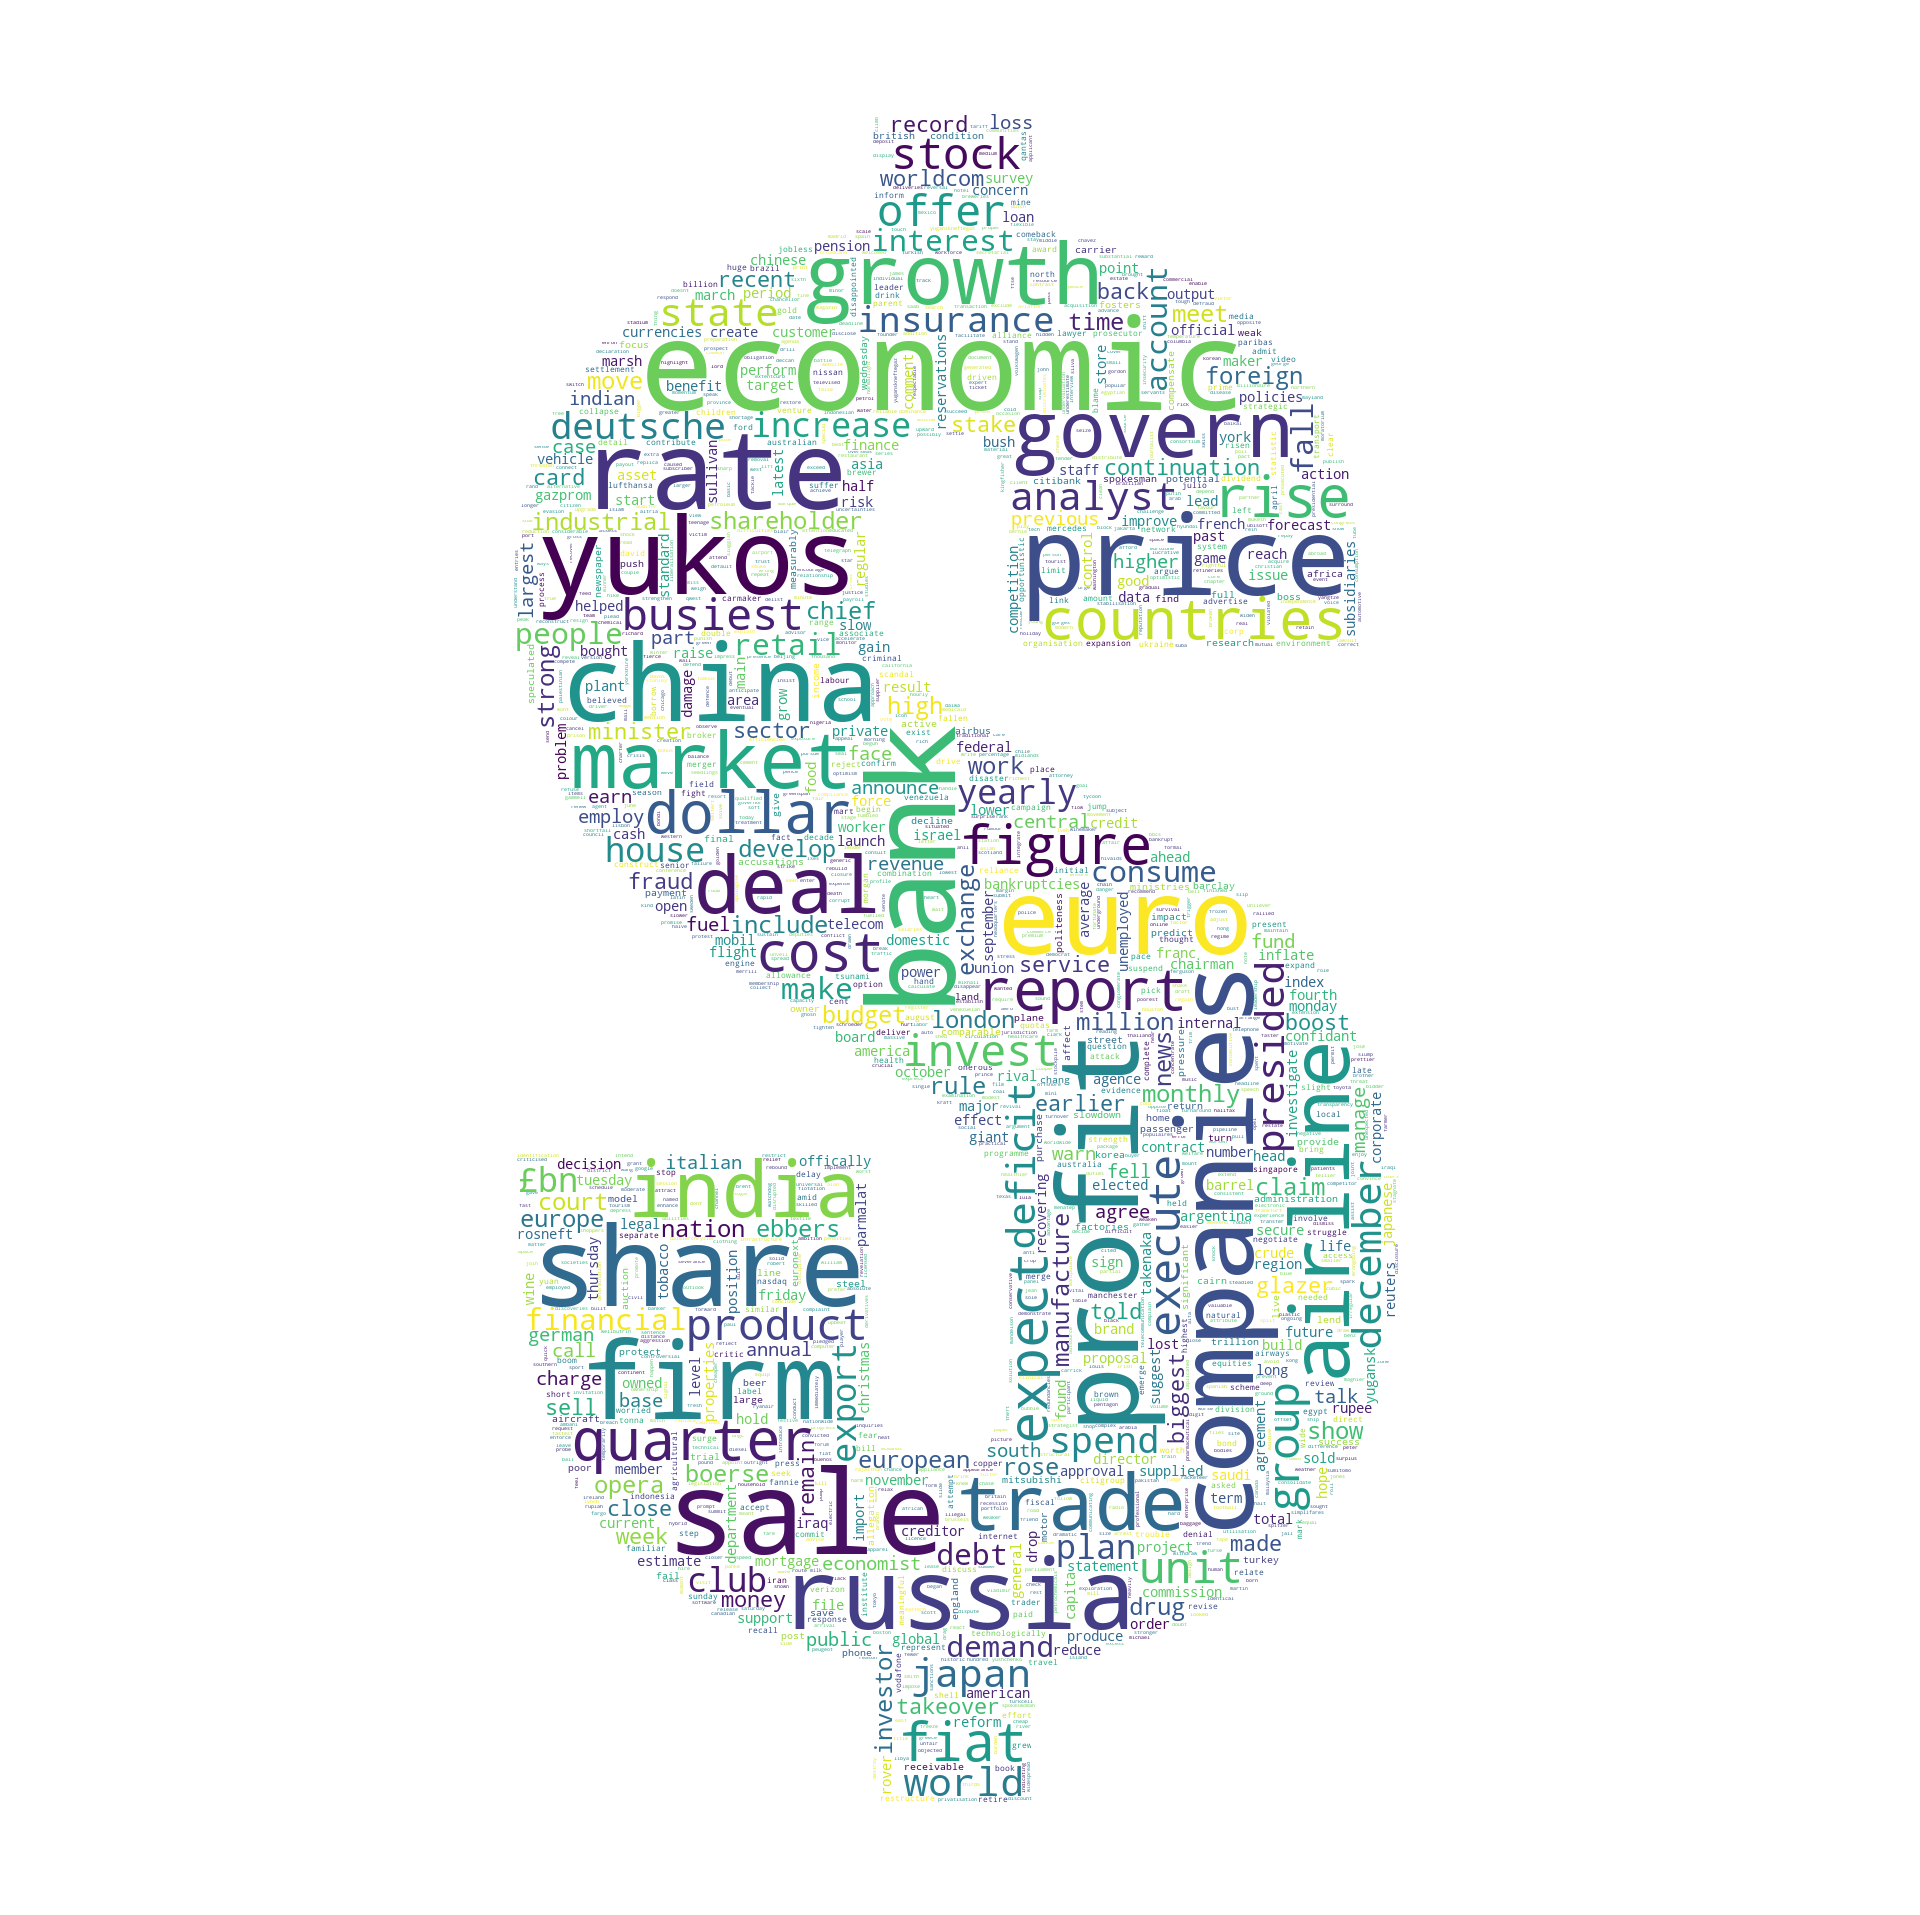
\includegraphics[width=\linewidth, height=10cm]{../graphs/dollarcloud.png}
	\caption{Wordcloud del corpus completo}
\end{figure}

Le parole più evidenti ben identificano il periodo storico degli articoli. Il periodo pre-crisi era caratterizzato da un clima di fiducia (profit, growth..) e dall'ascesa dei BRICS\footnote{Brasile, Russia, India, Cina, Sudafrica} (China, India..).
Le possibilità per analisi esplorative nel dettaglio sono infinite, ma vengono rimandate a successivi sviluppi per non deviare dal focus dell'articolo.
\newline
Si è scelto di concentrarsi su un tema molto presente negli articoli: lo scandalo Yukos\footnote{Nel 2003 Mikhail Khodorkovsky, CEO della Yukos, una delle più importanti aziende petrolifere russe di epoca post-sovietica, viene arrestato con le accuse di frode fiscale e bancarotta fraudolenta. Da quel momento al 2007, l'azienda viene liquidata.}\cite{yukos}: la parola ``Yukos" è associata al 64\% con la parola \textit{evasion}, e al 63\% con la parola \textit{court}, per esempio.

Verrà inoltre eseguita una sentiment analysis fra i documenti del cluster individuato corrispondenti allo scandalo Yukos, confrontandola con quella di un altro cluster.


I 12 cluster individuati, sono per l'appunto ben definiti: l'algoritmo dei k-medoidi unito alla dissimilarità del coseno ha prodotto ottimi risultati. I topics di ciascun cluster, individuati dagli autori per il confronto con il metodo automatizzato, sono riportati nella seguente tabella, unitamente alla loro NGD media:


\begin{table}[H]
	\begin{center}
		\begin{tabular}{|c|c|c|}
			\hline
			\textbf{Cluster} & \textbf{Keywords} & 	\textbf{Mean NGD} \\
			\hline
			\textbf{Cluster 1} & \{profit, sale, game, share, earn\} & 0.6419  \\ 
			\hline 
			\textbf{Cluster 2} & \{dollar, crude, deficit, bush, barrell\} & 0.4823 \\ 
			\hline 
			\textbf{Cluster 3} & \{yukos, russia, gazprom, court, action\} & 0.8301\\ 
			\hline 
			\textbf{Cluster 4} & \{fiat, italy, saab, opel, motor\} & 0.7555 \\ 
			\hline 
			\textbf{Cluster 5} & \{economy, growth, house, unemployed, inflation\} & 0.6056\\ 
			\hline 
			\textbf{Cluster 6} & \{china, yuan, japan, israel, islam\} & 0.7376 \\ 
			\hline 
			\textbf{Cluster 7} & \{lanka, disaster, people, indonesia, tsunami\} & 0.8734  \\ 
			\hline 
			\textbf{Cluster 8} & \{airline, india, quantas, airbus, lufthansa\} & 0.6679 \\ 
			\hline 
			\textbf{Cluster 9} & \{börse, deutsche, euronext, takeover, shareholder\} & 0.7223  \\ 
			\hline 
			\textbf{Cluster 10} & \{retail, sale, store, christmas, lvmh\} & 0.8551 \\ 
			\hline 
			\textbf{Cluster 11} & \{ebbers, fraud, verizon, qwest, lawyer\} & 0.7972\\ 
			\hline 
			\textbf{Cluster 12} & \{insurance, marsh, investigation, pension, plead\} & 0.4112  \\ 
			\hline 
		\end{tabular} 
		\caption{Topic estratti manualmente}
	\end{center}
\end{table}
È stata effettuata una sentiment analysis relativa ai documenti del primo cluster, ben rappresentativo dell'intero corpus, e una relativa ai documenti del terzo cluster, già citato in precedenza. Le differenze (e le similarità) sono notevoli:

\begin{figure}[H]
	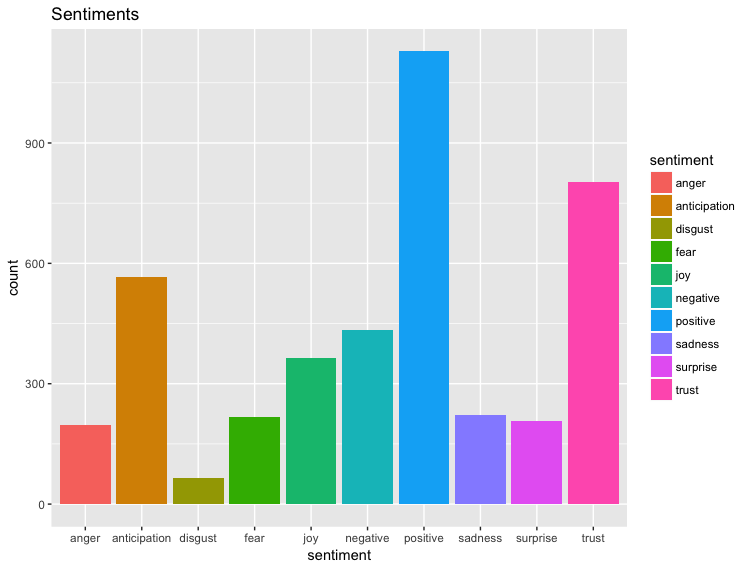
\includegraphics[width=\linewidth, height=10cm]{../graphs/sentiment_gr1.png}
	\caption{Sentiment Analysis Cluster 1}
\end{figure}

\begin{figure}[H]
	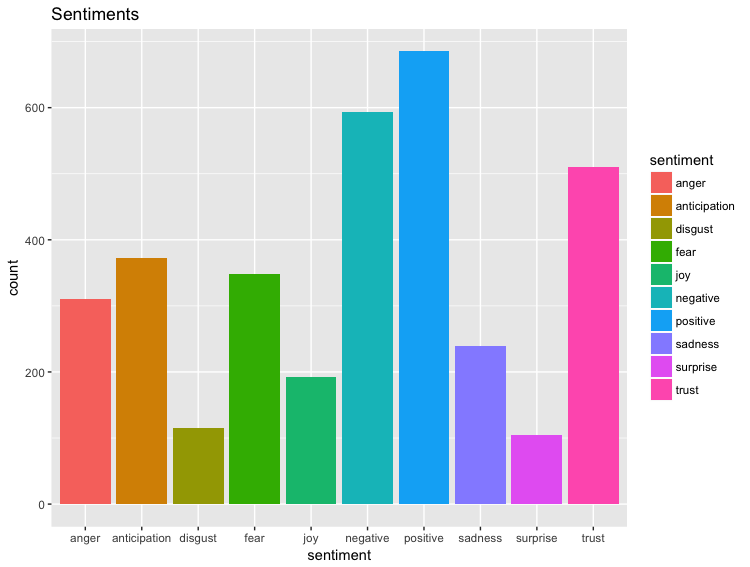
\includegraphics[width=\linewidth, height=10cm]{../graphs/sentiment_gr3.png}
	\caption{Sentiment Analysis Cluster 3}
\end{figure}

In entrambi i cluster, il sentimento prevalente è positivo, il che riflette il periodo generale pre-crisi, caratterizzato da una incrollabile fiducia nel sistema economico.
\newline
È pero evidente come nel cluster 3 ci sia molta più negatività, trattandosi comunque di documenti che trattavano temi quali evasione fiscale, e bancarotta. 


Per sviluppi futuri, sarebbe interessante selezionare altre compagnie/aziende ed effettuare una sentiment analysis relativa ai testi che le nominano per comprendere meglio il sentimento del mercato verso le stesse.

Passando al topic modeling effettuato con il modello LDA, la lista delle keywords indivuate automaticamente con le NGD medie è riportata nella tabella successiva:

\begin{table}[H]
	\begin{center}
	\begin{tabular}{|c|c|c|}
		\hline 
		\textbf{Topics} & \textbf{Keywords} & \textbf{Mean NGD} \\ 
		\hline 
		\textbf{Topic 1} & \{dollar, deficit, euro, budget, trade\} & 0.5121 \\ 
		\hline 
		\textbf{Topic 2} & \{bank, companies, firm, deal, financial\} & 0.2864 \\ 
		\hline 
		\textbf{Topic 3} & \{companies, firm, worldcom, ebbers, telecom\} & 0.773 \\ 
		\hline 
		\textbf{Topic 4} & \{yukos, russia, companies, court, firm\} & 0.6365 \\ 
		\hline 
		\textbf{Topic 5} & \{airline, cost, report, fuel, india\} & 0.6619 \\ 
		\hline 
		\textbf{Topic 6} & \{offer, deutsche, börse, share, london\} & 0.704 \\ 
		\hline 
		\textbf{Topic 7} & \{price, house, market, china, mortgage\} & 0.9843 \\ 
		\hline 
		\textbf{Topic 8} & \{economic, growth, rate, rise, figure\} & 0.3944 \\ 
		\hline 
		\textbf{Topic 9} & \{club, unit, glazer, invest, argentinah\} & 0.8455 \\ 
		\hline 
		\textbf{Topic 10} & \{economic, countries, govern, world, people\} & 0.6586 \\ 
		\hline 
		\textbf{Topic 11} & \{profit, sale, share, market, companies\}  & 0.6995 \\ 
		\hline 
	    \textbf{Topic 12} & \{companies, drug, call, firm, customer\} & 0.5654 \\ 
		\hline 
	\end{tabular} 	
	\caption{Topics estratti automaticamente}
	\end{center}
\end{table}
I topics estratti dal modello LDA in alcuni casi risultano sovrapponibili a quelli estratti manualmente o comunque chiari, mentre in altri sono un po' più fumosi. Per quanto riguarda la coerenza semantica, i 12 topics estratti manualmente presentano una NGD media di 0.7 mentre quelli automatici di 0.64. 
\newline
Il modello automatico fornisce una coerenza semantica addirittura maggiore del modello manuale, mostrandosi però meno capace ad individuare topics sempre ben definiti. Ciò porta a chiedersi se la NGD catturi tutta l'informazione possibile circa la coerenza semantica di due parole. Si rimandano le discussioni sulla metrica utilizzata all'ultimo paragrafo.
\newline
Per ultimo, è stato utilizzato IBM Watson sul primo testo del corpus:
{\footnotesize \blockquote{Ad sales boost Time Warner profit
	
	Quarterly profits at US media giant TimeWarner jumped 76\% to \$1.13bn (£600m) for the three months to December, from \$639m year-earlier.
	
	The firm, which is now one of the biggest investors in Google, benefited from sales of high-speed internet connections and higher advert sales. TimeWarner said fourth quarter sales rose 2\% to \$11.1bn from \$10.9bn. Its profits were buoyed by one-off gains which offset a profit dip at Warner Bros, and less users for AOL.
	
	Time Warner said on Friday that it now owns 8\% of search-engine Google. But its own internet business, AOL, had has mixed fortunes. It lost 464,000 subscribers in the fourth quarter profits were lower than in the preceding three quarters. However, the company said AOL's underlying profit before exceptional items rose 8\% on the back of stronger internet advertising revenues. It hopes to increase subscribers by offering the online service free to TimeWarner internet customers and will try to sign up AOL's existing customers for high-speed broadband. TimeWarner also has to restate 2000 and 2003 results following a probe by the US Securities Exchange Commission (SEC), which is close to concluding.
	
	Time Warner's fourth quarter profits were slightly better than analysts' expectations. But its film division saw profits slump 27\% to \$284m, helped by box-office flops Alexander and Catwoman, a sharp contrast to year-earlier, when the third and final film in the Lord of the Rings trilogy boosted results. For the full-year, TimeWarner posted a profit of \$3.36bn, up 27\% from its 2003 performance, while revenues grew 6.4\% to \$42.09bn. "Our financial performance was strong, meeting or exceeding all of our full-year objectives and greatly enhancing our flexibility," chairman and chief executive Richard Parsons said. For 2005, TimeWarner is projecting operating earnings growth of around 5\%, and also expects higher revenue and wider profit margins.
	
	TimeWarner is to restate its accounts as part of efforts to resolve an inquiry into AOL by US market regulators. It has already offered to pay \$300m to settle charges, in a deal that is under review by the SEC. The company said it was unable to estimate the amount it needed to set aside for legal reserves, which it previously set at \$500m. It intends to adjust the way it accounts for a deal with German music publisher Bertelsmann's purchase of a stake in AOL Europe, which it had reported as advertising revenue. It will now book the sale of its stake in AOL Europe as a loss on the value of that stake.
}}
Watson ha identificato come \textit{keywords}: \textit{Time Warner}, \textit{Time Warner profit}, \textit{higher advert sales}, \textit{AOL Eruope}, fra le altre, riuscendo inoltre a riconoscere le compagnie in esame e le persone citate accompagnando il riconoscimento con un link alle informazioni di ciascuna.
\section{Discussioni}
Il riconoscimento automatico dei topics si è mostrato valido: per quanto ancora non riesca a sintetizzare in maniera ``umana", la metrica utilizzata lo pone a un livello superiore alla sintesi manuale. Sarebbe interessante, da un lato, sviluppare il lavoro utilizzando metodi di topic extraction automatica più sofisticati, o con un approccio di tipo numerico come la \textit{Non-negative Matrix Factorization }(NMF); dall'altro, per la parte di riconoscimento manuale, sarebbero interessanti metodi di clustering più adeguati .
\newline
Sarebbe inoltre necessario sviluppare una metrica di coerenza semantica migliore, in quanto l'utilizzo della Normalized Google Distance desta non pochi dubbi. Per farlo, servirebbe però un corpus di riferimento strutturato e molto ampio, ma non è stato possibile reperirlo.


Ci si chiede, inoltre, quale possa essere l'obiettivo ultimo della sommarizzazione di un documento: se essa debba essere \textit{umanamente} comprensibile o se, come probabile, tale categorizzazione debba essere riconosciuta solamente da \textit{macchine}, per esempio per la ricerca di documenti in banche dati testuali. A quel punto probabilmente non sarà nemmeno più necessario che esse mantengano una certa coerenza semantica, rendendo necessario lo sviluppo di un nuovo metodo di valutazione.
\newline
IBM Watson d'altro canto, fornisce uno strumento accessibile a tutti e decisamente sofisticato e all'avanguardia per l'estrazione di informazioni da documenti. Nonostante si sia quasi raggiunto l'apice nell'ambito dell'\textit{information retrieval} con Watson, la sua natura proprietaria e privata rende comunque necessario uno sviluppo della ricerca nell'ambito dell'\textit{automatic topic modeling}.

\addcontentsline{toc}{chapter}{\refname}
\nocite{*}
\printbibliography

\end{document}
